% This file was created with tikzplotlib v0.10.1.
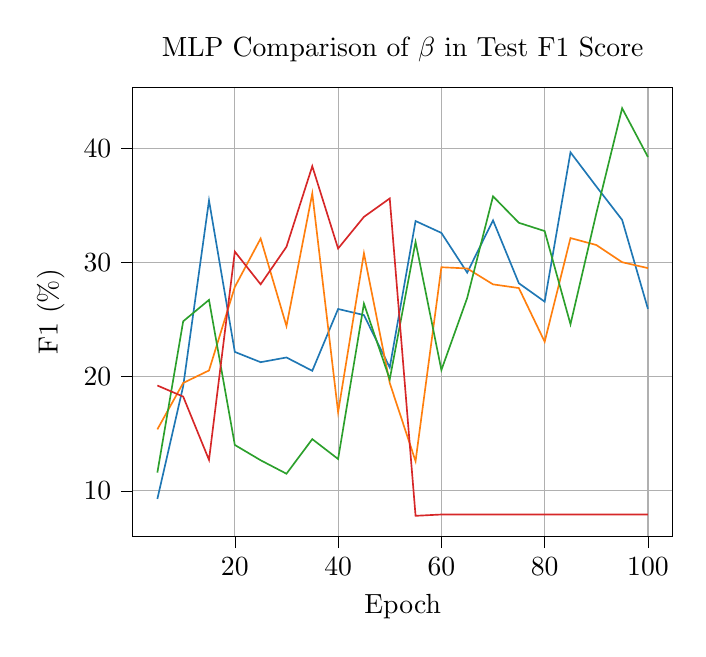
\begin{tikzpicture}

\definecolor{crimson2143940}{RGB}{214,39,40}
\definecolor{darkgray176}{RGB}{176,176,176}
\definecolor{darkorange25512714}{RGB}{255,127,14}
\definecolor{forestgreen4416044}{RGB}{44,160,44}
\definecolor{steelblue31119180}{RGB}{31,119,180}

\begin{axis}[
tick align=outside,
tick pos=left,
title={MLP Comparison of $\beta$ in Test F1 Score},
x grid style={darkgray176},
xlabel={Epoch},
xmajorgrids,
xmin=0.25, xmax=104.75,
xtick style={color=black},
y grid style={darkgray176},
ylabel={F1 (\%)},
ymajorgrids,
ymin=6.01843631159287, ymax=45.3289717895064,
ytick style={color=black}
]
\addplot [semithick, steelblue31119180]
table {%
5 9.28567520458969
10 19.166097885643
15 35.4595492031097
20 22.1766328280459
25 21.2755501635518
30 21.6898098538986
35 20.5200744419104
40 25.9417052633023
45 25.4059667449872
50 20.8159993893363
55 33.6540137015196
60 32.6128445456702
65 29.1325234472594
70 33.7135825381585
75 28.1991989700627
80 26.5834960795173
85 39.6751125629028
90 36.6867350709362
95 33.7549209532441
100 25.9494334039263
};
\addplot [semithick, darkorange25512714]
table {%
5 15.3858393972962
10 19.4559134525471
15 20.5501477650356
20 27.8723352117759
25 32.1182782908052
30 24.44546726661
35 36.0658174359138
40 16.8872085696282
45 30.821415191394
50 19.4512690423676
55 12.5983130596501
60 29.6024186476747
65 29.4944240485206
70 28.0996638323116
75 27.7772647520547
80 23.0697985516068
85 32.1602629440471
90 31.5518160462453
95 30.043110582696
100 29.5247873276621
};
\addplot [semithick, forestgreen4416044]
table {%
5 11.5936534837825
10 24.8595369301944
15 26.7382834100158
20 14.0197909892595
25 12.6777454171664
30 11.4962837123253
35 14.5298061890786
40 12.7872127872128
45 26.4095407392393
50 19.7733988338514
55 31.8233335603856
60 20.5890932650038
65 26.9129945961629
70 35.8201191303569
75 33.5000870430073
80 32.7734220002176
85 24.6022868668876
90 34.3194365570498
95 43.5421292677831
100 39.2667104554277
};
\addplot [semithick, crimson2143940]
table {%
5 19.2319159899513
10 18.2586644125106
15 12.7090301003344
20 30.9720387757794
25 28.102935346119
30 31.3931084070498
35 38.4597547539238
40 31.242574541074
45 34.0179769563157
50 35.6344963171445
55 7.80527883331622
60 7.92000792000792
65 7.92000792000792
70 7.92000792000792
75 7.92000792000792
80 7.92000792000792
85 7.92000792000792
90 7.92000792000792
95 7.92000792000792
100 7.92000792000792
};
\end{axis}

\end{tikzpicture}
